\documentclass{article}
\usepackage[utf8]{inputenc}
\usepackage{listings}
\usepackage{multimedia} % to embed movies in the PDF file
\usepackage{graphicx}
\usepackage{comment}
\usepackage[english]{babel}
\usepackage{amsmath}
\usepackage{amsfonts}
\usepackage{subfigure}
\usepackage{wrapfig}
\usepackage{multirow}
\usepackage{tikz}
\usepackage{verbatim}
%!TEX root = main.tex



\newcommand{\eref}[1]{\mbox{\rm(\ref{#1})}}
\newcommand{\tref}[1]{\mbox{\rm\ref{#1}}}
\newcommand{\set}[2]{\left\{ #1 \; : \; #2 \right\} }
\newcommand{\deq}{\raisebox{0pt}[1ex][0pt]{$\stackrel{\scriptscriptstyle{\rm def}}{{}={}}$}}

\newcommand {\DS} {\displaystyle}

\newcommand{\real}{\mathbb{R}}



\newcommand {\half} {\mbox{$\frac{1}{2}$}}
\newcommand{\force}{{\mathbf{f}}}
\newcommand{\strain}{{\boldsymbol{\varepsilon}}}
\newcommand{\stress}{{\boldsymbol{\sigma}}}
\renewcommand{\div}{{\boldsymbol{\nabla}}}

\newcommand {\cA} {{\cal A}}
\newcommand {\cB} {{\cal B}}
\newcommand {\cC} {{\cal C}}
\newcommand {\cD} {{\cal D}}
\newcommand {\cE} {{\cal E}}
\newcommand {\cK} {{\cal K}}
\newcommand {\cL} {{\cal L}}
\newcommand {\cP} {{\cal P}}
\newcommand {\cQ} {{\cal Q}}
\newcommand {\cR} {{\cal R}}
\newcommand {\cV} {{\cal V}}
\newcommand {\cW} {{\cal W}}
\newcommand {\CC} {{\cal C}}
\newcommand {\CD} {{\cal D}}
\newcommand {\CH} {{\cal H}}
\newcommand {\CS} {{\cal S}}
\newcommand {\CU} {{\cal U}}
\newcommand {\CY} {{\cal Y}}



\newcommand{\bzero}{\mathbf{0}}
\newcommand{\ba}{\mathbf{a}}
\newcommand{\bb}{\mathbf{b}}
\newcommand{\bc}{\mathbf{c}}
\newcommand{\bd}{\mathbf{d}}
\newcommand{\be}{\mathbf{e}}
\newcommand{\bg}{\mathbf{g}}
\newcommand{\bh}{\mathbf{h}}
\newcommand{\bl}{\mathbf{l}}
\newcommand{\bn}{\mathbf{n}}
\newcommand{\bp}{\mathbf{p}}
\newcommand{\bq}{\mathbf{q}}
\newcommand{\br}{\mathbf{r}}
\newcommand{\bs}{\mathbf{s}}
\newcommand{\bt}{\mathbf{t}}
\newcommand{\bu}{\mathbf{u}}
\newcommand{\bv}{\mathbf{v}}
\newcommand{\bw}{\mathbf{w}}
\newcommand{\bx}{\mathbf{x}}
\newcommand{\by}{\mathbf{y}}
\newcommand{\bz}{\mathbf{z}}
\newcommand{\bA}{{\mathbf A}}
\newcommand{\bB}{\mathbf{B}}
\newcommand{\bC}{\mathbf{C}}
\newcommand{\bD}{\mathbf{D}}
\newcommand{\bE}{\mathbf{E}}
\newcommand{\bF}{\mathbf{F}}
\newcommand{\bG}{\mathbf{G}}
\newcommand{\bH}{\mathbf{H}}
\newcommand{\bI}{\mathbf{I}}
\newcommand{\bJ}{\mathbf{J}}
\newcommand{\bK}{\mathbf{K}}
\newcommand{\bL}{\mathbf{L}}
\newcommand{\bM}{\mathbf{M}}
\newcommand{\bN}{\mathbf{N}}
\newcommand{\bO}{\mathbf{O}}
\newcommand{\bP}{\mathbf{P}}
\newcommand{\bQ}{\mathbf{Q}}
\newcommand{\bR}{\mathbf{R}}
\newcommand{\bS}{\mathbf{S}}
\newcommand{\bU}{\mathbf{U}}
\newcommand{\bV}{\mathbf{V}}
\newcommand{\bW}{\mathbf{W}}
\newcommand{\bX}{\mathbf{X}}
\newcommand{\bY}{\mathbf{Y}}
\newcommand{\bZ}{\mathbf{Z}}

\newcommand{\bgamma}{{\boldsymbol{\gamma}}}
\newcommand{\bmu}{{\boldsymbol{\mu}}}
\newcommand{\bkappa}{{\boldsymbol{\kappa}}}
\newcommand{\blambda}{{\boldsymbol{\lambda}}}
\newcommand{\bLambda}{{\boldsymbol{\Lambda}}}
\newcommand{\bpi}{{\boldsymbol{\pi}}}
\newcommand{\bPi}{{\boldsymbol{\Pi}}}
\newcommand{\btheta}{{\boldsymbol{\theta}}}
\newcommand{\bTheta}{{\boldsymbol{\Theta}}}
\newcommand{\bSigma}{{\boldsymbol{\Sigma}}}





\title{AMATH 567 Homework 2}
\author{Cade Ballew \#2120804}
\date{October 13, 2021}

\begin{document}

\maketitle

\section{Problem 1 (1.2.11)}
Say that we are given a straight line in the complex plane and wish to determine what the stereographic projection of its points looks like. The geometric definition of the steroeographic projection says that we map a point in the complex plane to the point where the line between the north pole of the sphere and the point in the complex plane intersects the sphere. If we generalize this to a collection of points, our line in the complex plane and the north pole of the sphere define a plane (a point and a line in 3 dimensions define a plane). The intersection of this plane and the sphere is a circle that, of course, passes through the north pole of the sphere, so this is precisely what lines in the complex plane project to.    

\section{Problem 2 (1.3.5)} 
The definition of differentiability is that a function $f$ is differentiable at a point $z\in\mathbb{C}$ if 
\begin{equation*}
    \lim_{\Delta z \to 0}\frac{f(z+\Delta z)-f(z)}{\Delta z}
\end{equation*}
exists. Let $f(z)=\Re(z)$ and write this limit as 
\begin{equation*}
    \lim_{(\Delta x,\Delta y) \to (0,0)}\frac{\Re(x+\Delta x,y+\Delta y)-\Re(x,y)}{\Delta x + i \Delta y}
\end{equation*}
where $z=x+iy$ and $\Delta z= \Delta x+i\Delta y$. Then, our limit becomes
\begin{equation*}
    \lim_{(\Delta x,\Delta y) \to (0,0)}\frac{x+\Delta x-x}{\Delta x + i \Delta y} = \lim_{(\Delta x,\Delta y) \to (0,0)}\frac{\Delta x}{\Delta x + i \Delta y}.
\end{equation*}
However, this limit does not exist, because it changes depending on what direction we approach from; if we consider $(\Delta x,\Delta y)=(\Delta x, 0)$ as our approach direction, the limit is clearly 1, but if we consider $(\Delta x,\Delta y)=(0, \Delta y)$, the limit is clearly 0. Thus, $\Re(z)$ is not differentiable anywhere, because this analysis did not depend on our choice of $z$. \\
Similarly, if we consider $f(z)=\Im(z)$, 
\begin{equation*}
\begin{split}
    \lim_{\Delta z \to 0}\frac{f(z+\Delta z)-f(z)}{\Delta z} = \lim_{(\Delta x,\Delta y) \to (0,0)}\frac{\Im(x+\Delta x,y+\Delta y)-\Im(x,y)}{\Delta x + i \Delta y}\\=
    \lim_{(\Delta x,\Delta y) \to (0,0)}\frac{y+\Delta y-y}{\Delta x + i \Delta y} = \lim_{(\Delta x,\Delta y) \to (0,0)}\frac{\Delta y}{\Delta x + i \Delta y}.
\end{split}
\end{equation*}
As before, the limit does not exist; if we consider $(\Delta x,\Delta y)=(\Delta x, 0)$ as our approach direction, the limit is clearly 0, but if we consider $(\Delta x,\Delta y)=(0, \Delta y)$, the limit is clearly $-i$. Thus, $\Im(z)$ is also nowhere differentiable.
\section{Problem 3 (1.3.11)}
\subsection{Part a}
Consider the differential equation 
\begin{equation*}
    \frac{d^3w}{dt^3}-k^3w=0 
\end{equation*}
for $t\in\real$ and some constant $k\in\real$.\\
Its characteristic polynomial is $D^3-k^3$, so we wish to solve $D^3-k^3=0$ for $D$. We use the concept of roots of unity to solve this which gives $D_1=\sqrt[3]{k}=k$, $D_2=\sqrt[3]{k}e^{2\pi i/3}=k(-1/2+i\sqrt{3}/2)=-k/2+ik\sqrt{3}/2$, and $D_3=\sqrt[3]{k}e^{4\pi i/3}=k(-1/2-i\sqrt{3}/2)=-k/2-ik\sqrt{3}/2$. We can now write that general solution as we would in any introductory undergraduate course in ODEs. Namely, 
\begin{equation*}
    w(t) = c_1e^{kt}+c_2e^{-kt/2}\cos(k\sqrt{3}/2)+c_3e^{-kt/2}\sin(k\sqrt{3}/2).
\end{equation*}
\section{Problem 4}
We wish to find all complex roots of the function $\cos z$. We begin by writing out the definition of the complex cosine and factoring
\begin{equation*}
    \cos z= \frac{e^{iz}+e^{-iz}}{2}=\frac{e^{-iz}(e^{2iz}+1)}{2}.
\end{equation*}
Thus, $\cos z=0$ iff either $e^{-iz}=0$ or $e^{2iz}+1=0$. The former can never occur, because the complex exponential can never be zero by definition (because $e^{x+iy}=e^z(\cos y+i\sin y)$ and $\cos y=\sin y=0$ does not hold for any real $y$). Thus, we solve
\begin{equation*}
    e^{2iz}=-1=e^{i\pi}=e^{i(\pi+2\pi k)} 
\end{equation*}
for any $k\in\mathbb{Z}$. This gives that $2z=\pi+2\pi k$, so the solutions of $\cos z$ are precisely $z=\pi/2+\pi k$ for any $k\in\mathbb{Z}$.\\
We know from class (and by definition) that $\cosh z=\cos iz$. Thus, the zeroes of $\cosh z$ are precisely the zeroes of $\cos iz$, meaning that $iz=\pi/2+\pi k$ which occurs iff $z=-i(\pi/2+\pi k)$. Thus, the zeroes of $\cosh z$ are $z=i(-\pi/2+\pi k)$ for any $k\in\mathbb{Z}$.
\section{Problem 5}
We consider the function $f_\epsilon=1/(\epsilon^2+z^2)$ for $z\in\mathbb{C}/\{i\epsilon,-i\epsilon\}$ and $\epsilon=1,0.5,0.1,0.01$. Using MATLAB, we plot these functions on a grid $-1\leq\Re (z)\leq1$ and $-1\leq\Im (z)\leq1$ with distance 0.01 between consecutive points and a log-scale on the vertical axis and obtain the following plots:\\
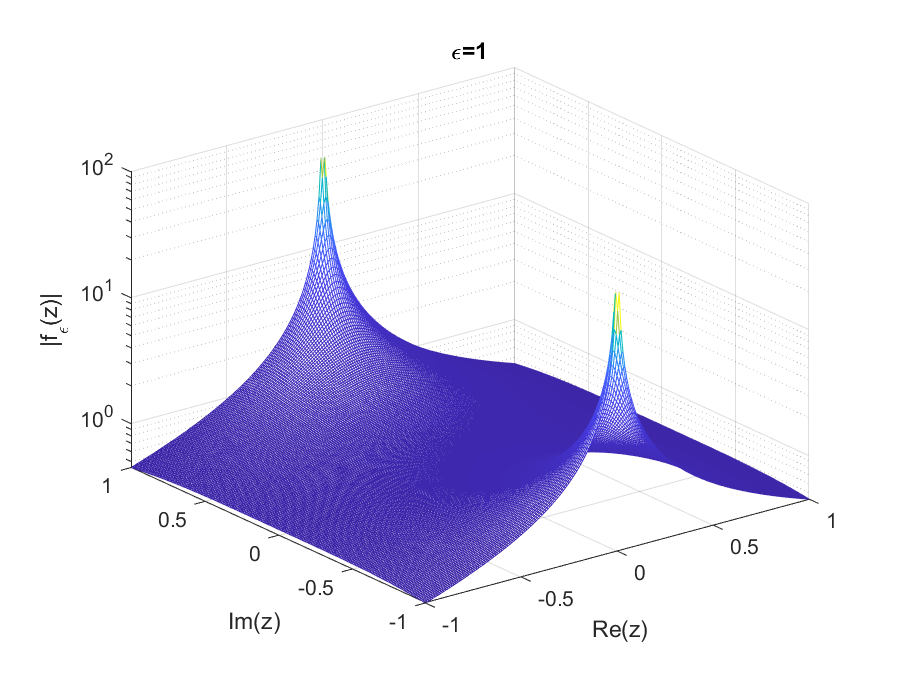
\includegraphics[scale=0.55]{1.eps}
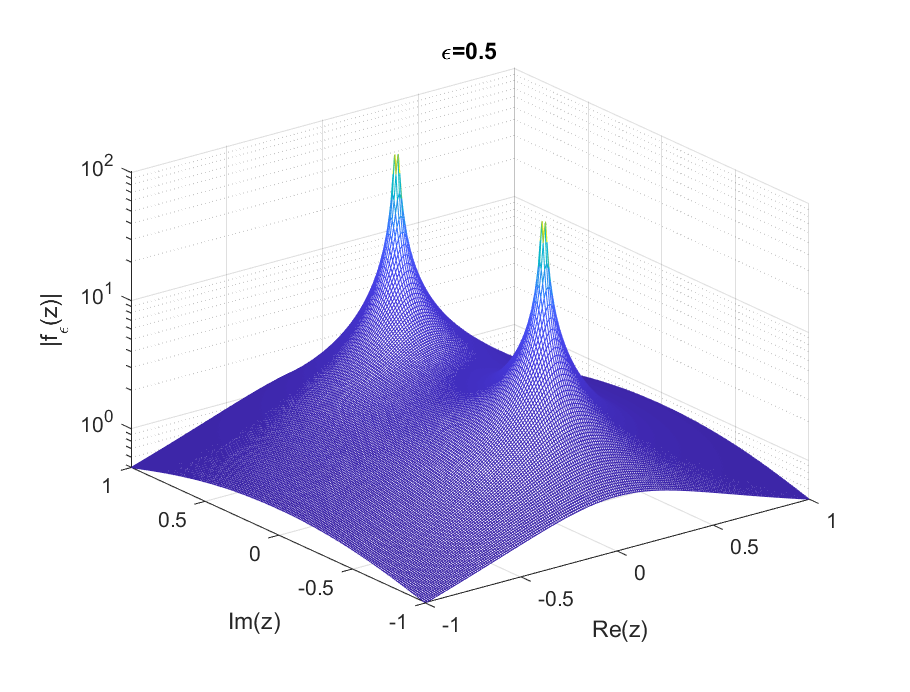
\includegraphics[scale=0.55]{2.eps}
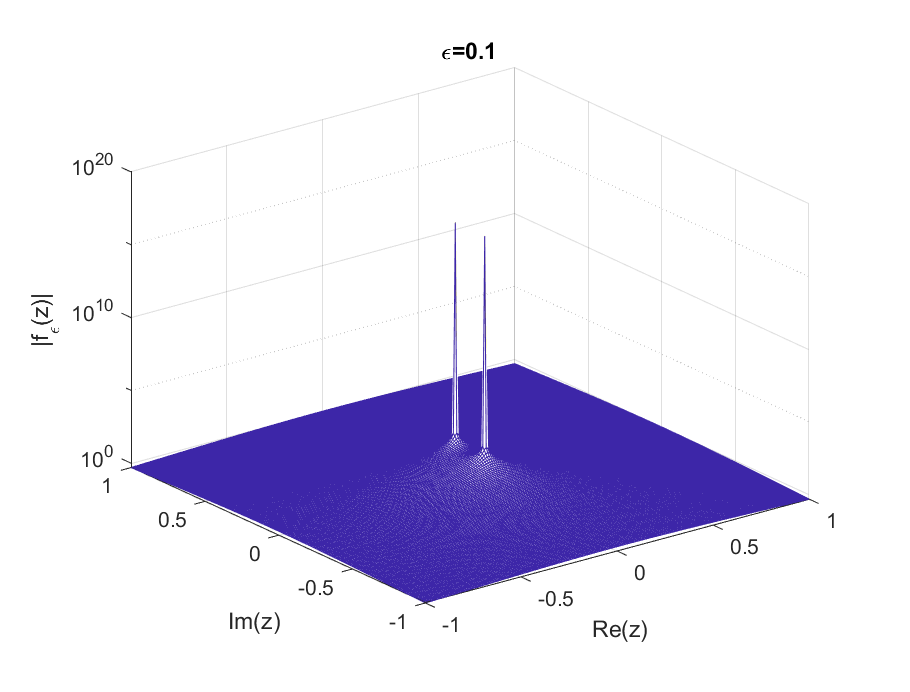
\includegraphics[scale=0.55]{3.eps}
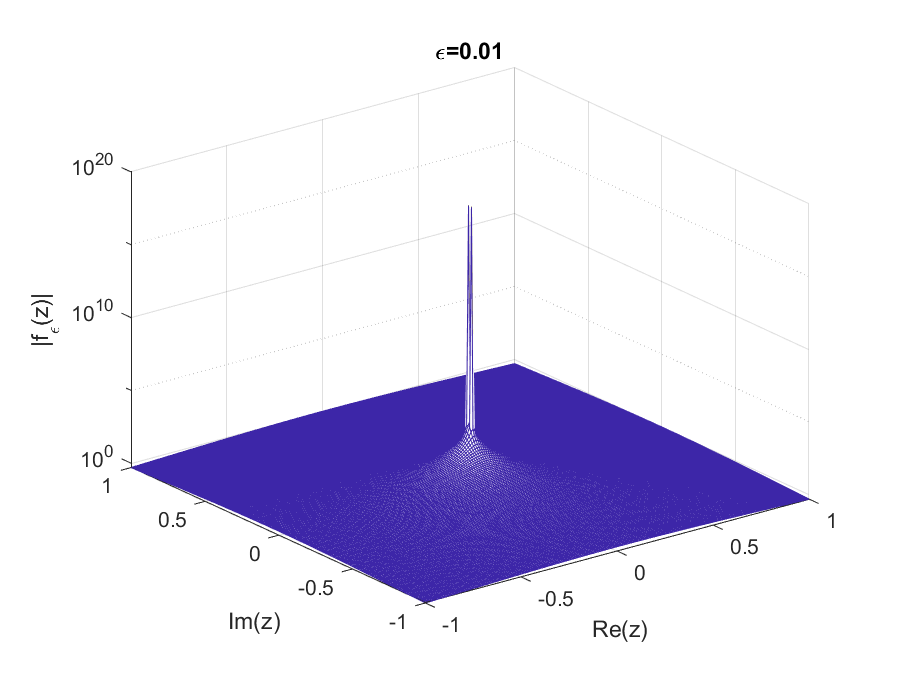
\includegraphics[scale=0.55]{4.eps}\\
To see how the function on the real line is impacted, we now include plots of the functions $f_\epsilon(x)=1/(\epsilon^2+x^2)$ for $x\in\real$:\\
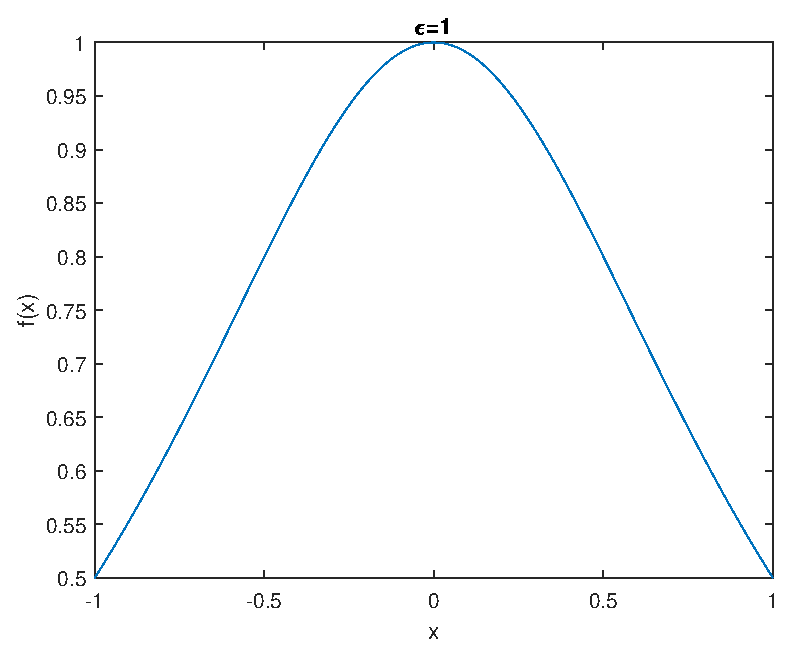
\includegraphics[scale=0.55]{real1.eps}
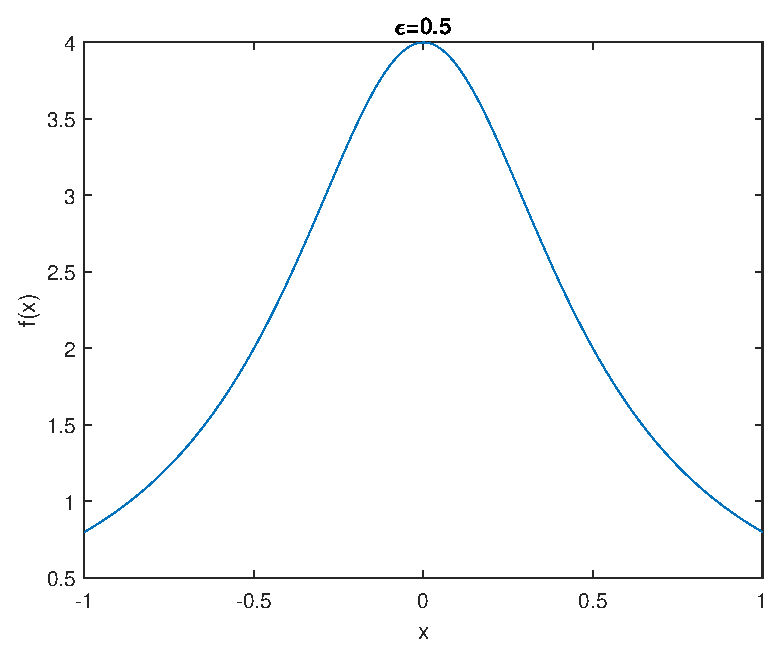
\includegraphics[scale=0.55]{real2.eps}
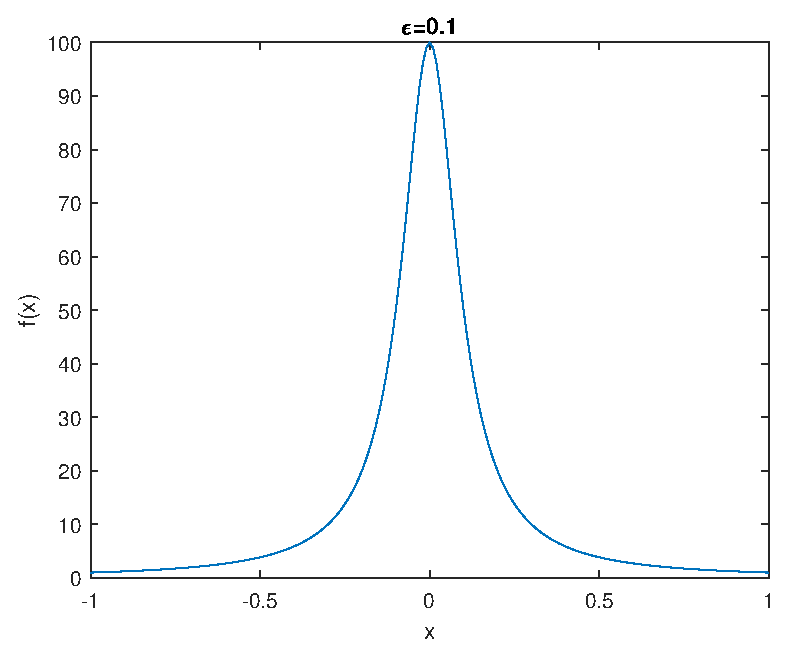
\includegraphics[scale=0.55]{real3.eps}
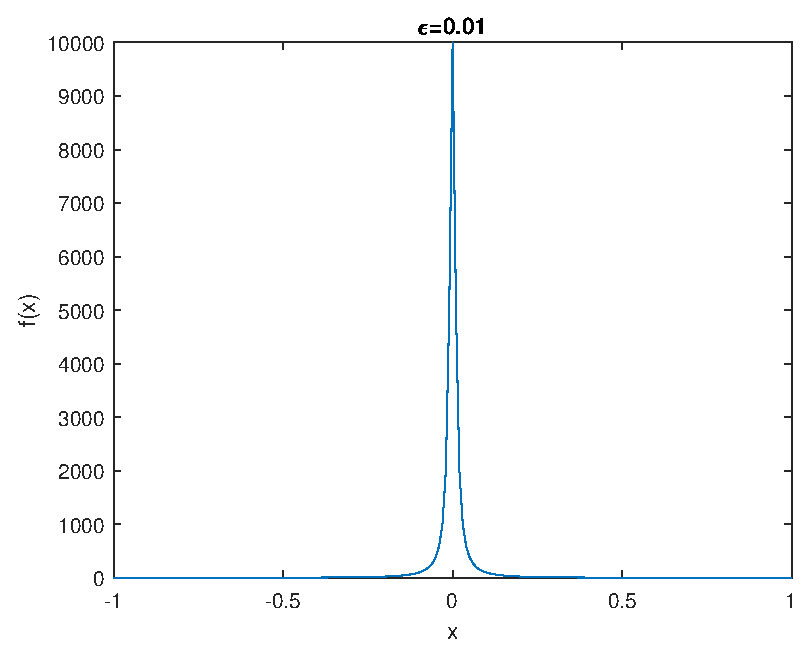
\includegraphics[scale=0.55]{real4.eps}\\
We can clearly see from our surface plots that as the singularities move closer the origin, the points in close proximity to them correspond to function values of greater magnitude. These singularities have 0 real part for any $\epsilon>0$, so $x=0$ is the point on the real line that will be most impacted by them. This impact will also become more prominent as $\epsilon\to 0$, because the singularities approach the real line. This explains why in our plots of the corresponding function on the real line, the point $x=0$ starts to resemble a discontinuity as $\epsilon\to 0$ ($x=0$ is getting closer to an actual discontinuity in the complex plane). 
\section{Problem 6 (2.1.1)}
\subsection{Part a}
Consider the function $f(x,y)=x-iy+1$. Then $f(x,y)=u(x,y)+iv(x,y)$ with $u(x,y)=x+1$, $v(x,y)=-y$. We compute $u_x=1$ and $v_y=-1$ which are not equal for any $x,y\in\real$, so $f(x,y)$ does not satisfy the Cauchy-Riemann equations.
\subsection{Part b}
Now, consider $f(x,y)=y^3-3x^2y+i(x^3-3xy^2+2)$. Then, $u(x,y)=y^3-3x^2y$ and $v(x,y)=x^3-3xy^2+2$. We compute $u_x=6xy=v_y$ and $u_y=3y^2-3x^2=-v_x$, so $f$ satisfies the Cauchy-Riemann equations. \\
Now, note that $(y-ix)^3=y^3-3ixy^2-3x^2y+ix^3$, so $f(x,y)=(y-ix)^3+2i$. If $z=x+iy$, $y-ix=-iz$ which gives that $(y-ix)^3+2i=(-iz)^3+2i=-i^3z^3+2i=i(z^3+2)$. Thus, $f(z)=i(z^3+2)$ is the analytic function of $z$ corresponding to $f(x,y)$.
\subsection{Part c}
Now, take $f(x,y)=e^y(\cos x+i\sin y)$. Then, $u(x,y)=e^y\cos x$ and $v(x,y)=e^y\sin y$. We compute $u_y=e^y\cos x$ and $-v_x=0$. $u_y=-v_x$ holds only when $\cos x=0$. Also, $u_x=-e^y\sin x$ and $v_y = e^y\sin y +e^y\cos y$, so $u_x=v_y$ also holds only when $\pm e^y = e^y(\sin y+\cos y)$ (because $\sin x=\pm$ 1 when $\cos x=0$). Thus, in order for the Cauchy-Riemann equations to be satisfied, we must have that $\cos x=0$ and $\sin y+\cos y=\pm1$. This only occurs at discrete $(x,y)$, so the Cauchy-Riemann equations do not hold in general, and we cannot find an analytic function of $z$.

\section{Problem 7 (2.1.7)}
Consider $\phi$ as $\phi(u(x,y),v(x,y))$. Then, by the chain rule, 
\begin{equation*}
    \frac{\partial\phi}{\partial x}=\frac{\partial u}{\partial x}\frac{\partial\phi}{\partial u}+\frac{\partial v}{\partial x}\frac{\partial\phi}{\partial v}
\end{equation*}
Similarly, 
\begin{equation*}
    \frac{\partial\phi}{\partial y}=\frac{\partial u}{\partial y}\frac{\partial\phi}{\partial u}+\frac{\partial v}{\partial y}\frac{\partial\phi}{\partial v}
\end{equation*}
Then, by the chain and product rules,
\begin{equation*}
\begin{split}
    \frac{\partial^2\phi}{\partial x^2}&=
    \frac{\partial}{\partial x}(\frac{\partial\phi}{\partial x})\\&=
    \frac{\partial}{\partial x}(\frac{\partial u}{\partial x}\frac{\partial\phi}{\partial u}+\frac{\partial v}{\partial x}\frac{\partial\phi}{\partial v})\\&=
    \frac{\partial^2 u}{\partial x^2}\frac{\partial \phi}{\partial u}+\frac{\partial u}{\partial x}*(\frac{\partial }{\partial x}(\frac{\partial \phi}{\partial u}))+\frac{\partial^2 v}{\partial x^2}\frac{\partial \phi}{\partial v}+\frac{\partial v}{\partial x}*(\frac{\partial }{\partial x}(\frac{\partial \phi}{\partial v}))\\&=
    \frac{\partial^2 u}{\partial x^2}\frac{\partial \phi}{\partial u}+\frac{\partial u}{\partial x}*(\frac{\partial u}{\partial x}\frac{\partial^2 \phi}{\partial u^2}+\frac{\partial v}{\partial x}\frac{\partial^2 \phi}{\partial u \partial v})+\frac{\partial^2 v}{\partial x^2}\frac{\partial \phi}{\partial v}+\frac{\partial v}{\partial x}*(\frac{\partial  v}{\partial x}\frac{\partial^2 \phi}{\partial v^2}+\frac{\partial u}{\partial x}\frac{\partial^2 \phi}{\partial u \partial v})\\&=
    \frac{\partial^2 u}{\partial x^2}\frac{\partial \phi}{\partial u}+(\frac{\partial u}{\partial x})^2\frac{\partial^2 \phi}{\partial u^2}+\frac{\partial u}{\partial x}\frac{\partial v}{\partial x}\frac{\partial^2 \phi}{\partial u \partial v}+\frac{\partial^2 v}{\partial x^2}\frac{\partial \phi}{\partial v}+(\frac{\partial v}{\partial x})^2\frac{\partial^2 \phi}{\partial v^2}+\frac{\partial u}{\partial x}\frac{\partial v}{\partial x}\frac{\partial^2 \phi}{\partial u \partial v}\\&=
    \frac{\partial^2 u}{\partial x^2}\frac{\partial \phi}{\partial u}+(\frac{\partial u}{\partial x})^2\frac{\partial^2 \phi}{\partial u^2}+2\frac{\partial u}{\partial x}\frac{\partial v}{\partial x}\frac{\partial^2 \phi}{\partial u \partial v}+\frac{\partial^2 v}{\partial x^2}\frac{\partial \phi}{\partial v}+(\frac{\partial v}{\partial x})^2\frac{\partial^2 \phi}{\partial v^2}.
\end{split}
\end{equation*}
Then, we use the second Cauchy-Riemann equation to substitute $v_x=-u_y$ and find
\begin{equation*}
\begin{split}
    \frac{\partial^2\phi}{\partial x^2}&=
    \frac{\partial^2 u}{\partial x^2}\frac{\partial \phi}{\partial u}+(\frac{\partial u}{\partial x})^2\frac{\partial^2 \phi}{\partial u^2}+2\frac{\partial u}{\partial x}(-\frac{\partial u}{\partial y})\frac{\partial^2 \phi}{\partial u \partial v}+(\frac{\partial}{\partial x}(-\frac{\partial u}{\partial y}))\frac{\partial \phi}{\partial v}+(-\frac{\partial u}{\partial y})^2\frac{\partial^2 \phi}{\partial v^2}\\&=
    \frac{\partial^2 u}{\partial x^2}\frac{\partial \phi}{\partial u}-\frac{\partial^2 u}{\partial x\partial y}\frac{\partial \phi}{\partial v}+(\frac{\partial u}{\partial x})^2\frac{\partial^2 \phi}{\partial u^2}-2\frac{\partial u}{\partial x}\frac{\partial u}{\partial y}\frac{\partial^2 \phi}{\partial u \partial v}+(\frac{\partial u}{\partial y})^2\frac{\partial^2 \phi}{\partial v^2}
\end{split}
\end{equation*}
as desired. \\
Similarly, 
\begin{equation*}
\begin{split}
    \frac{\partial^2\phi}{\partial y^2}&=
    \frac{\partial}{\partial y}(\frac{\partial\phi}{\partial y})\\&=
    \frac{\partial}{\partial y}(\frac{\partial u}{\partial y}\frac{\partial\phi}{\partial u}+\frac{\partial v}{\partial y}\frac{\partial\phi}{\partial v})\\&=
    \frac{\partial^2 u}{\partial y^2}\frac{\partial \phi}{\partial u}+\frac{\partial u}{\partial y}*(\frac{\partial }{\partial y}(\frac{\partial \phi}{\partial u}))+\frac{\partial^2 v}{\partial y^2}\frac{\partial \phi}{\partial v}+\frac{\partial v}{\partial y}*(\frac{\partial }{\partial y}(\frac{\partial \phi}{\partial v}))\\&=
    \frac{\partial^2 u}{\partial y^2}\frac{\partial \phi}{\partial u}+\frac{\partial u}{\partial y}*(\frac{\partial u}{\partial y}\frac{\partial^2 \phi}{\partial u^2}+\frac{\partial v}{\partial y}\frac{\partial^2 \phi}{\partial u \partial v})+\frac{\partial^2 v}{\partial y^2}\frac{\partial \phi}{\partial v}+\frac{\partial v}{\partial y}*(\frac{\partial  v}{\partial y}\frac{\partial^2 \phi}{\partial v^2}+\frac{\partial u}{\partial y}\frac{\partial^2 \phi}{\partial u \partial v})\\&=
    \frac{\partial^2 u}{\partial y^2}\frac{\partial \phi}{\partial u}+(\frac{\partial u}{\partial y})^2\frac{\partial^2 \phi}{\partial u^2}+\frac{\partial u}{\partial y}\frac{\partial v}{\partial y}\frac{\partial^2 \phi}{\partial u \partial v}+\frac{\partial^2 v}{\partial y^2}\frac{\partial \phi}{\partial v}+(\frac{\partial v}{\partial y})^2\frac{\partial^2 \phi}{\partial v^2}+\frac{\partial u}{\partial y}\frac{\partial v}{\partial y}\frac{\partial^2 \phi}{\partial u \partial v}\\&=
    \frac{\partial^2 u}{\partial y^2}\frac{\partial \phi}{\partial u}+(\frac{\partial u}{\partial y})^2\frac{\partial^2 \phi}{\partial u^2}+2\frac{\partial u}{\partial y}\frac{\partial v}{\partial y}\frac{\partial^2 \phi}{\partial u \partial v}+\frac{\partial^2 v}{\partial y^2}\frac{\partial \phi}{\partial v}+(\frac{\partial v}{\partial y})^2\frac{\partial^2 \phi}{\partial v^2}\\&=
    \frac{\partial^2 u}{\partial y^2}\frac{\partial \phi}{\partial u}+(\frac{\partial u}{\partial y})^2\frac{\partial^2 \phi}{\partial u^2}+2\frac{\partial u}{\partial y}\frac{\partial u}{\partial x}\frac{\partial^2 \phi}{\partial u \partial v}+(\frac{\partial}{\partial y}(\frac{\partial u}{\partial x}))\frac{\partial \phi}{\partial v}+(\frac{\partial u}{\partial x})^2\frac{\partial^2 \phi}{\partial v^2}\\&=
    \frac{\partial^2 u}{\partial y^2}\frac{\partial \phi}{\partial u}+\frac{\partial^2 u}{\partial x \partial y}\frac{\partial \phi}{\partial v}+(\frac{\partial u}{\partial y})^2\frac{\partial^2 \phi}{\partial u^2}+2\frac{\partial u}{\partial x}\frac{\partial u}{\partial y}\frac{\partial^2 \phi}{\partial u \partial v}+(\frac{\partial u}{\partial x})^2\frac{\partial^2 \phi}{\partial v^2}
\end{split}
\end{equation*}
when we use the first Cauchy-Riemann equation to substitute $v_y=u_x$. \\
Now, we have that
\begin{equation*}
\begin{split}
    \Delta_{x,y}\phi&=
    \frac{\partial^2\phi}{\partial x^2}+\frac{\partial^2\phi}{\partial y^2}\\&=
    \frac{\partial^2 u}{\partial x^2}\frac{\partial \phi}{\partial u}+\frac{\partial^2 u}{\partial y^2}\frac{\partial \phi}{\partial u}+(\frac{\partial u}{\partial x})^2\frac{\partial^2 \phi}{\partial u^2}+(\frac{\partial u}{\partial x})^2\frac{\partial^2 \phi}{\partial v^2}+(\frac{\partial u}{\partial y})^2\frac{\partial^2 \phi}{\partial u^2}+(\frac{\partial u}{\partial y})^2\frac{\partial^2 \phi}{\partial v^2}\\&=
    (\frac{\partial^2 u}{\partial x^2}+\frac{\partial^2 u}{\partial x^2})\frac{\partial \phi}{\partial u}+\bigg((\frac{\partial u}{\partial x})^2+(\frac{\partial u}{\partial y})^2\bigg)(\frac{\partial^2 \phi}{\partial u^2}+\frac{\partial^2 \phi}{\partial v^2})\\&=
    (\frac{\partial^2 u}{\partial x^2}+\frac{\partial^2 u}{\partial x^2})\frac{\partial \phi}{\partial u}+(u_x^2+u_y^2)(\frac{\partial^2 \phi}{\partial u^2}+\frac{\partial^2 \phi}{\partial v^2}).
\end{split}
\end{equation*}
We know from the text (and lecture) that the real part of a complex analytic function is itself a harmonic function, thus $u$ is a harmonic function of $x$ and $y$, meaning that $\frac{\partial^2 u}{\partial x^2}+\frac{\partial^2 u}{\partial x^2}=0$ and
\begin{equation*}
    \Delta_{x,y}=(u_x^2+u_y^2)(\frac{\partial^2 \phi}{\partial u^2}+\frac{\partial^2 \phi}{\partial v^2})
\end{equation*}
as a result. \\
Finally, we know that $f'(z)=u_x+i v_x = u_x-i u_y$ from the derivation of and the second Cauchy-Riemann equation. Thus, $|f'(z)|^2=u_x^2+u_y^2$, meaning that we can write
\begin{equation*}
\begin{split}
    \Delta_{x,y}\phi&=
    \frac{\partial^2\phi}{\partial x^2}+\frac{\partial^2\phi}{\partial y^2}=(u_x^2+u_y^2)(\frac{\partial^2 \phi}{\partial u^2}+\frac{\partial^2 \phi}{\partial v^2})\\&=
    |f'(z)|^2\Delta_{u,v}\phi,
\end{split}
\end{equation*}
as desired.
\section{Problem 8}
Consider $f(z)=|z|^2=x^2+y^2=u(x,y)+iv(x,y)$ where $u(x,y)=x^2+y^2$ and $v(x,y)=0$. Theorem 2.1.1 in the text states that $f$ is differentiable at a point $z=x+iy$ iff $u_x,u_y,v_x,v_y$ are continuous and satisfy the Cauchy-Riemann equations at $z=x+iy$. We first compute $u_x=2x$, $u_y=2y$, $v_x=0$, $v_y=0$; clearly, these functions are continuous for any $z\in\mathbb{C}$. However, the Cauchy-Riemann equations hold iff $2x=0$ and $2y=0$, meaning that they hold iff $z=x+iy=0$. Thus, by theorem 2.1.1, $f(z)=|z|^2$ is differentiable at $z=0$ but nowhere else.

\section{Problem 9}
To derive the polar form of the Cauchy-Riemann equation we first consider the identity $r^2=x^2+y^2$ and differentiate implicitly with respect to $x$. This gives that $2r\frac{\partial r}{\partial x}=2x$ because y is independent with respect to x. Similarly, we differentiate $\tan\theta=\frac{y}{x}$ implicitly with respect to $x$ and get that $\sec^2\theta\frac{\partial \theta}{\partial x}=-\frac{y}{x^2}$. We then find that
\begin{equation*}
    \frac{\partial r}{\partial x} = \frac{x}{r} = \frac{r\cos\theta}{r} = \cos\theta
\end{equation*}
and
\begin{equation*}
    \frac{\partial\theta}{\partial x} = \cos^2\theta\frac{-y}{x^2} = \cos^2\theta\frac{-r\sin\theta}{r^2\cos^2\theta}=-\frac{\sin\theta}{r}
\end{equation*}
By this and the chain rule, we find the differential relationship
\begin{equation*}
    \frac{\partial}{\partial x} = \frac{\partial}{\partial r}\frac{\partial r}{\partial x}+\frac{\partial}{\partial \theta}\frac{\partial \theta}{\partial x} = \cos\theta\frac{\partial}{\partial r}-\frac{\sin\theta}{r}\frac{\partial}{\partial \theta}
\end{equation*}
Similarly, we can differentiate the same equations implicitly with respect to $y$ and get 
\begin{equation*}
    \frac{\partial r}{\partial y} = \frac{y}{r} = \frac{r\sin\theta}{r} = \sin\theta
\end{equation*}
and
\begin{equation*}
    \frac{\partial\theta}{\partial x} = \cos^2\theta\frac{1}{x} = \cos^2\theta\frac{1}{r\cos\theta}=\frac{\cos\theta}{r}
\end{equation*}
which give that
\begin{equation*}
    \frac{\partial}{\partial y} = \frac{\partial}{\partial r}\frac{\partial r}{\partial y}+\frac{\partial}{\partial \theta}\frac{\partial \theta}{\partial y} = \sin\theta\frac{\partial}{\partial r}+\frac{\cos\theta}{r}\frac{\partial}{\partial \theta}
\end{equation*}
We can apply these relations to the original Cauchy-Riemann equations to get 
\begin{equation}\label{CR1}
    u_x=\cos\theta\frac{\partial u}{\partial r}-\frac{\sin\theta}{r}\frac{\partial u}{\partial \theta}=\sin\theta\frac{\partial v}{\partial r}+\frac{\cos\theta}{r}\frac{\partial v}{\partial \theta}=v_y
\end{equation}
and 
\begin{equation}\label{CR2}
    u_y=\sin\theta\frac{\partial u}{\partial r}+\frac{\cos\theta}{r}\frac{\partial u}{\partial \theta}=-\cos\theta\frac{\partial v}{\partial r}+\frac{\sin\theta}{r}\frac{\partial v}{\partial \theta}=-v_x
\end{equation}
If we multiply \eqref{CR1} by $\cos\theta$ and \eqref{CR2} by $\sin\theta$ and sum, we get 
\begin{equation*}
    \cos^2\theta\frac{\partial u}{\partial r}+\sin^2\theta\frac{\partial u}{\partial r}=\frac{\cos^2\theta}{r}\frac{\partial v}{\partial \theta}+\frac{\sin^2\theta}{r}\frac{\partial v}{\partial \theta}
\end{equation*}
which when using the fact that $\cos^2\theta+\sin^2\theta=1$ gives that $\frac{\partial u}{\partial r}=\frac{1}{r}\frac{\partial v}{\partial \theta}$.
Similarly, if we multiply \eqref{CR1} by $\sin\theta$ and \eqref{CR2} by $-\cos\theta$ and sum, we get
\begin{equation*}
    -\frac{\sin^2\theta}{r}\frac{\partial u}{\partial \theta}-\frac{\cos^2\theta}{r}\frac{\partial u}{\partial \theta}=\sin^2\theta\frac{\partial v}{\partial r}+\cos^2\theta\frac{\partial v}{\partial r}
\end{equation*}
which again gives the desired result $\frac{\partial v}{\partial r}=-\frac{1}{r}\frac{\partial u}{\partial \theta}$ when using the identity $\cos^2\theta+\sin^2\theta=1$.
Thus, we have derived the polar Cauchy-Riemann equations from their original form.
\end{document}
